\section{Application}
\label{sec:inference:app}
% \todo[inline]{entire code in appendix? => Yes, todos, cleanup}
% \todo[inline]{write that row vectors are meant if not specified otherwise? => probably not necessary, easily spottable due to the context}

The inference application is written in Python 3 and the complete listing can be found in appendix \ref{app:inference_application}.
% Although Python is not known for extremely fast execution times there are several tricks which make it possible to run almost as fast as a native app.
% Although Python is not known for extremely fast execution times, there are some tricks that allow it to run almost as fast as a native application.
Although Python is not known for extremely fast execution times, it allows for fast and easy development.
% Furthermore, several methods are used that allow the inference application to run almost as fast as a native application.
Furthermore, several methods are used to improve the speed of execution.
This allows the inference application to run almost as fast as a native application.
% Additionally

% overview (not a chapter)
% routine of the app
% 1. init cam / 2. ...
% This section explains the procedure of the inference application shown in figure \ref{fig:procedure_inference_app}.
This section describes the procedure of the inference application shown in figure \ref{fig:procedure_inference_app}.
% After the initialization of the \acrshort{dpu} and the camera, the frame acquisition is stared.
After the initialization of the \acrshort{dpu} and the camera, the image acquisition is stared.
% Once a throw has been detected
Once a throw has been completed, the frames are processed and several predictions are made.
These predictions are then weighted and the result is displayed on the screen.
% Lastly, the global variables are reset and the image acquisition is started again.
% In a last step, the global variables are reset to their original values.
Finally, the global variables are reset to their original values.
% This completes the cycle and the image acquisition is started again.
% This completes the sequence and the image acquisition is started again.
This completes the never-ending sequence and the image acquisition is started again.

\begin{figure}
  \centering
  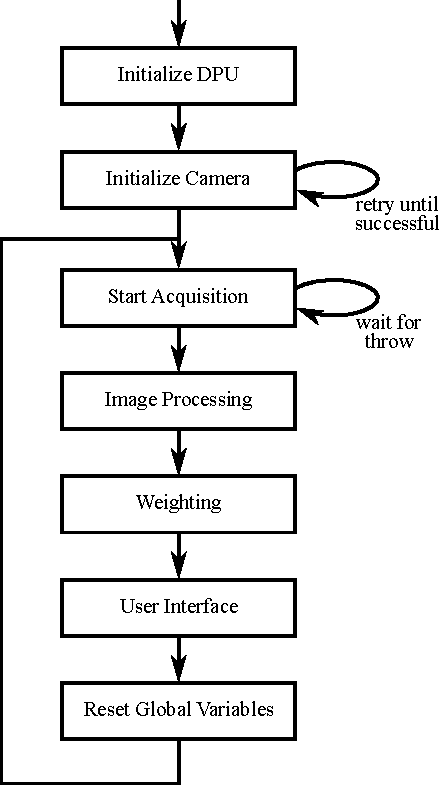
\includegraphics[width=0.5\textwidth]{program_flow} % done: draw and add procedure graphics
  \caption{Procedure of the inference application}
  \label{fig:procedure_inference_app}
\end{figure}

% ------------------------------------------------------------------------------------------------------------------------------
\subsection{Initialization}
\label{subsec:inference:app:initialization}
% \todo[inline]{not finished yet}

The initialization process consists of two parts:
\begin{enumerate}
  \item Initializing the \acrshort{dpu}
  \item Initializing the camera
\end{enumerate}

% -----------------------------------------
\paragraph{Initializing the \acrshort{dpu}}
% The initialization procedure of the \acrshort{dpu} consists of loading the quantized \acrshort{cnn} model and setting up the \acrshort{dpu}.
% The initialization procedure of the \acrshort{dpu} consists of loading the \acrshort{dpu} and loading the quantized \acrshort{cnn} model.
The initialization procedure of the \acrshort{dpu} consists of loading and setting up the \acrshort{dpu}.
% explain those two:
% from dnndk import n2cube
% from pynq_dpu import DpuOverlay
This is done with the two Python packages \texttt{pynq\_dpu} and \texttt{dnndk}.
% The \texttt{pynq\_dpu} package provides a class to load the desired \acrshort{dpu} and the \texttt{dnndk} package is a thin wrapper around the \acrshort{n2cube} library.
The \texttt{pynq\_dpu} package provides a class to load the desired \acrshort{dpu}.
The \texttt{dnndk} package contains the \texttt{n2cube} module, which is a thin wrapper around the \acrshort{n2cube} library and allows to interface with the implemented \acrshort{dpu} \cite{}. % todo: cite https://github.com/Xilinx/DPU-PYNQ

% init DPU
% done with overlays
% loads the overlay (architecture ad weights of the neural network)
% The first step consists of loading the quantized \acrshort{cnn} model in the form of an overlay.
% The first step consists of loading the quantized \acrshort{cnn} model with the overlay files \texttt{dpu.bit}, \texttt{dpu.hwh} and \texttt{dpu.xclbin}.
The first step consists of loading the \acrshort{dpu} with the three overlay files \texttt{dpu.bit}, \texttt{dpu.hwh} and \texttt{dpu.xclbin}.
% The first part is to initialize the \acrshort{dpu}.
% These contain the architecture and the weights of the quantized \acrshort{cnn} model.
These files contain the bitstream to flash the \acrshort{dpu} to the \acrlong{pl} and the necessary information to interface with it.

% (thin wrapper around N2Cube)
The second step is to set up the \acrshort{dpu}.
% For this reason, the \acrshort{n2cube} function \texttt{n2cube.dpuLoadKernel} is used to load a so-called kernel.
Therefore, the \acrshort{n2cube} function \texttt{n2cube.dpuLoadKernel} is used to load a so-called kernel.
This kernel contains the architecture and the weights of the quantized \acrshort{cnn} model.
% These contain the architecture and the weights of the quantized \acrshort{cnn} model.

% ---------------------------------
\paragraph{Initializing the Camera}
To initialize the camera, the camera library has to be loaded first.
% explain import ctypes shortly
This is done with the Python package \texttt{ctypes}, which provides C compatible data types and allows to call functions of shared libraries \cite{}. % todo: cite https://docs.python.org/3/library/ctypes.html
Once loaded, the various mutator functions of the camera library are used to control settings such as the frame rate and the exposure time (see section \ref{sec:inference:camera_library}).

% init camera
% - wait until successful (show error in the UI)
Finally, the camera is initialized by calling the function \texttt{libcamera.initialize}.
The return code of this function is used to check, whether the initialization was successful.
% If an initialization error occurs, the initialization function is simply called again.
% An initialization error of the camera is shown on the bootsplash screen.
If an initialization error occurs, an error message is shown on the bootsplash screen.
The initialization function is called until it succeeds, which is listed in appendix \ref{app:inference_application} on lines \ref{lst:ln:camera_init1}--\ref{lst:ln:camera_init2}
% the initialization function is simply called again.
% An initialization 
% To avoid a reboot of the entire system if
This is to avoid a reboot of the entire system if the camera is not plugged in during the startup of the application.

% ------------------------------------------------------------------------------------------------------------------------------
\subsection{Image Acquisition}
\label{subsec:inference:app:image_acquisition}
\todo[inline]{not quite finished yet}

The camera library features several accessor functions to access the global variables.
% This allows the use of parallelism.



The image acquisition 


% thread -> Concurrency
% process -> Parallelism
The Python interpreter features a \acrfull{gil}, which allows only one thread to execute code \cite{}. % todo: cite https://opensource.com/article/17/4/grok-gil
% The Python standard library contains two packages to realize thread-based and process-based parallelism.
However, the Python standard library contains two packages to realize thread-based and process-based parallelism.
On the one hand, thread-based parallelism can be realized with the \texttt{threading} package \cite{}. % todo: cite https://docs.python.org/3/library/threading.html
On the other hand, process-based parallelism can be realized with the \texttt{multiprocessing} package, which spawns a new process for each task \cite{}. % todo: cite https://docs.python.org/3/library/multiprocessing.html
Different threads run concurrently, which means that different tasks are executed at the same time, but not simultaneously.
Different processes can run simultaneously on different cores of the processor \cite{}. % todo: cite https://medium.com/swift-india/concurrency-parallelism-threads-processes-async-and-sync-related-39fd951bc61d

% The problem with the \texttt{multiprocessing} package is, that different processes are not allowed to access different memory regions
The problem with the \texttt{multiprocessing} package is, that different processes do not share memory.
% and thus the entire initialization of the camera would also have to be done in the process
% Therefore, it would not be possible to poll the values of the global variables
% This makes the polling of the global variables impossible and therefore the image processing could only begin after the image acquisition is done.
This makes it impossible to poll the global variables, and therefore, the image processing can only begin after the image acquisition is complete.

% explain that this is used:
% from threading import Thread
Fortunately, in this case the \texttt{threading} package is ideal.
The \texttt{ctypes} package releases the \acrshort{gil} before calling a C function \cite{}. % todo: cite https://docs.python.org/3.3/library/ctypes.html
This allows the \texttt{libcamera.start\_acquisition} function to run simultaneously in a thread on another processor core.

However, practical tests have shown that the embedded system is not powerful enough to acquire and process frames at the same time.
% As soon as any other processor heavy computation starts, the
% As soon as any other processor-intensive calculation starts, the Camera Library starts losing images.
The camera library starts to drop frames as soon as another processor-intensive task, such as the image processing, is started.


% still benefitial because of
% - pDevice->GetRemoteNode("AcquisitionStop")->Execute();
% - pDataStream->StopAcquisition();






% Camera
% start acquisition
% - multi processing
% reset variables
% terminate




% ## our application

% - explain how it could have been done in C++ or Python
%   - python wins, because it's easier for quick prototyping
%   - there is no (noticable) performance loss when using Python, since the same N2Cube lib is used with a minimal Python wrapper around it (this is possible with ctypes, since cpython is used [most common])
%     - there is also no perfomance loss for the camera application because of the same reason (ctypes-implementation)
%   - explain both processes in detail (C++ with the CMake file, which requires the sysroot with all the headers and shared objects [libraries])
%     - maybe talk about the docker conatainer which could be used but is not ideal if you add stuff to the sysroot, weh creating your own PwtaLinux with opencv + baumer...
%   - explain that the C++ and Python API are very similar and so a conversion between the two is not really difficult








% ------------------------------------------------------------------------------------------------------------------------------
\subsection{Image Processing}
\label{subsec:inference:app:image_processing}
% \todo[inline]{not finished yet}

The image classification chain consists of five serialized steps:
% resizing, ...
\begin{enumerate}
  \item Getting the raw Baumer \texttt{BayerRG8} frame
  \item Converting the color space
  \item Resizing the frame
  \item Normalizing the pixel values
  \item Running inference
\end{enumerate}

% Steps one to four are for the image preprocessing and step five does the actual image classification.
Steps one to four serve for image preprocessing and step five for the actual image classification.

% It makes no sense to evaluate all frames of a throw as this would strongly impact the time required to classify an image.
% However, it makes no sense to evaluate all frames of a throw, as this would strongly impact the required classification time of a throw.
However, it makes no sense to evaluate all frames of a throw, as this would strongly impact the total required classification time.
% Furthermore, the classification accuracy of the \acrshort{cnn} model is quite high and therefore a low amount of frames is sufficient to make an accurate prediction.
Furthermore, the classification accuracy of the \acrshort{cnn} model is quite high, so that a small number of frames is sufficient to make an accurate prediction.

Analysing the dataset reveals the ideal number of frames to consider to cover all frames of at least \SI{80}{\percent} of all throws.
% Analysing the dataset reveals the ideal number of frames that should be considered to cover all frames of at least \SI{80}{\percent} of all throws.
% plot that shows with 22 frames everything is good
% Histogram (Bimodal) => no, a histogram is used for continuous data!
% Figure \ref{fig:frame_distribution} shows the distribution of the number of frames per throw $f(n)$.
% The distribution of the number of frames per throw $f(x)$ is shown in figure \ref{fig:frame_distribution}.
% The distribution of the number of throws with $x$ frames $f(x)$ is shown in figure \ref{fig:frame_distribution}.
% The distribution of the number of frames per throw $f(x)$ is shown in figure \ref{fig:distribution}.
The empirical distribution of the number of frames per throw $f(x)$ is shown in figure \ref{fig:distribution}.
% The normalized summation of the frame distribution $F(n)$ is calculated with the following equation:
% Figure \ref{fig:frame_distribution_summation} shows the normalized summation of the frame distribution $F(n)$, which can be calculated with equation \ref{eq:frame_distribution_summation}.
% The empirical distribution function
% The discrete cumulative distribution function of
% The empirical cumulative distribution function of
% Figure \ref{fig:frame_distribution_summation} shows the empirical cumulative distribution function $F(n)$, which can be calculated with equation \ref{eq:frame_distribution_summation}.
% Figure \ref{fig:cumulative_distribution} shows the empirical cumulative distribution function $F(x)$, which can
% Figure \ref{fig:cumulative_distribution} shows the empirical cumulative distribution function $F(x)$ of the distribution $f(x)$.
This distribution is used to derive the empirical cumulative distribution function $F(x)$ shown in figure \ref{fig:cumulative_distribution}.
% It shows that with only \num{22} frames over \SI{80}{\percent} of all throws
It shows that \SI{80}{\percent} of all throws consist of \num{22} frames or less.
For this reason, a maximum of \num{22} frames are processed by the image classification chain.
% Therefore, a maximum of \num{22} frames are processed by the image classification chain.

\begin{figure}
  \centering
  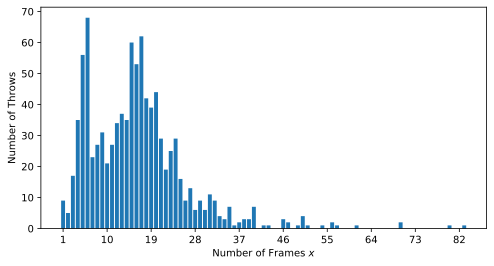
\includegraphics[width=\textwidth]{distribution}
  \caption{Distribution of the number of frames per throw $f(x)$}
  \label{fig:distribution}
\end{figure}

\begin{figure}
  \centering
  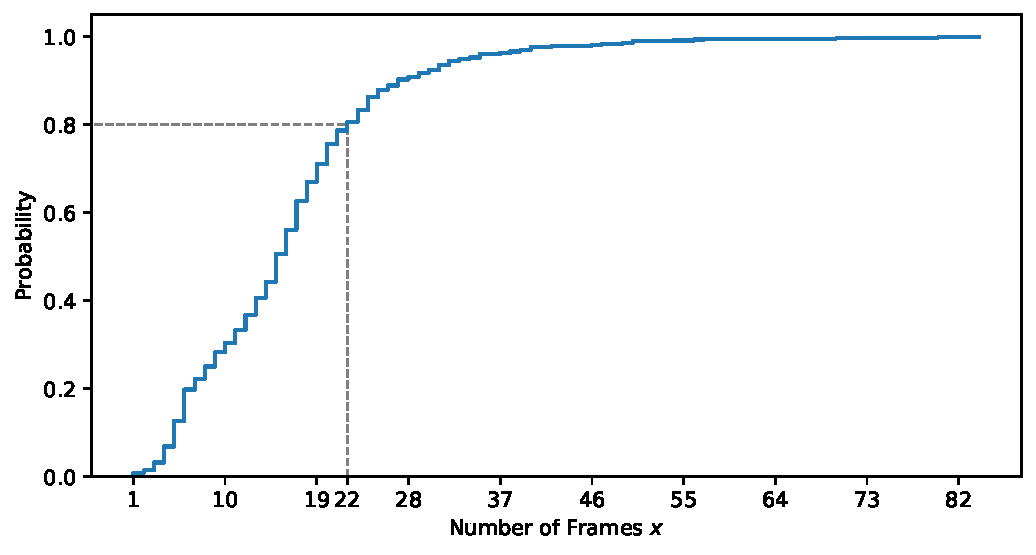
\includegraphics[width=\textwidth]{cumulative_distribution}
  % \caption{Normalized summation of the frame distribution $F(n)$}
  \caption{Empirical cumulative distribution function $F(x)$}
  \label{fig:cumulative_distribution}
\end{figure}

% -----------------------------
\paragraph{Image Preprocessing}
The image preprocessing is is listed in appendix \ref{app:inference_application} on lines \ref{lst:ln:image_preprocessing1}--\ref{lst:ln:image_preprocessing2}.
% explain that those are used: cv2 / numpy
% It uses the NumPy and \acrshort{opencv} packages.
For this purpose the Python packages NumPy and \acrshort{opencv} are used.
Those packages are just thin Python wrappers around the native-implemented libraries and therefore very performant.

The first step consists of getting the raw Baumer \texttt{BayerRG8} frame from memory and store it in a NumPy array.
This is done with the help of a pointer to the raw frame.

In a second step, the color space is converted from raw Baumer \texttt{BayerRG8} to \acrshort{bgr}.
% The conversion uses the \acrshort{opencv} function \texttt{cvtColor} with the color space conversion code \texttt{cv2.COLOR\_BayerBG2BGR} \cite{}. % todo: cite https://docs.opencv.org/3.4.3/d7/d1b/group__imgproc__misc.html#ga397ae87e1288a81d2363b61574eb8cab
The conversion uses the \acrshort{opencv} function \texttt{cvtColor}, which operates on NumPy arrays.
The required color space conversion code is set to \texttt{cv2.COLOR\_BayerBG2BGR} \cite{}. % todo: cite https://docs.opencv.org/3.4.3/d7/d1b/group__imgproc__misc.html#ga397ae87e1288a81d2363b61574eb8cab
This odd conversion code results from the fact that Baumer and \acrshort{opencv} use different naming schemes.
The Baumer \texttt{BayerRG} format corresponds to the \acrshort{opencv} \texttt{BayerBG} format.

The third step is to resize the frames with the \acrshort{opencv} function \texttt{cv2.resize}.
This function is supplied with three arguments: the NumPy array that represents the image, the desired output image size and the interpolation method \cite{}. % todo: cite https://docs.opencv.org/3.4.3/da/d54/group__imgproc__transform.html#ga47a974309e9102f5f08231edc7e7529d
% The used interpolation method used is the same one as during the training.
% The interpolation method used is the same as during training (see section \ref{subsec:training_of_the_cnn:dataset:augmentation}).
% The nearest-neighbor interpolation method is used, the same as during training (see section \ref{subsec:training_of_the_cnn:dataset:augmentation}).
For performance reasons, the nearest-neighbor interpolation method is used (see section \ref{subsec:training_of_the_cnn:dataset:augmentation}).

The last step consists of normalizing the individual pixel values to the range between \numrange{0}{1}, just as it was done during training (see section \ref{sec:training_of_the_cnn:training}).
% The individual pixel values have to be normalized to the range between \numrange{0}{1}, as the same was done during the training (see section \ref{sec:training_of_the_cnn:training}).

% ------------------------------
\paragraph{Image Classification}
% explain the calls to run inference
% The actual image classification is done with the \acrshort{n2cube} function \texttt{n2cube.dpuRunTask}, as shown in appendix \ref{app:inference_application} on line \ref{lst:ln:image classification}.
The actual image classification is done with the \acrshort{n2cube} function \texttt{n2cube.dpuRunTask}, which uses the quantized \acrshort{cnn} model to make a prediction on the supplied input image.
This is shown in appendix \ref{app:inference_application} on line \ref{lst:ln:image_classification}.

% these are the output values of the CNN (from the output layer)
% The output values $\boldsymbol{z}$ of the \acrshort{cnn} model
The output values of the quantized \acrshort{cnn} model are denoted by the output vector

\begin{equation}
  \boldsymbol{z} =
  \begin{bmatrix}
    z_1 & z_2 & \dots & z_c \\
  \end{bmatrix}.
  \label{eq:output_vector}
\end{equation}

The values of the output vector $\boldsymbol{z}$ are 8-bit signed integers which represent a fixed-point format.
% on these the softmax function is used to get probabilities (read more theory about this!)
% To normalize the the output vector to a probability distribution, the softmax function is used.
% The softmax function is used to normalize the values of the output vector to a discrete probability distribution over the target classes.
To normalize the values of the output vector to a discrete probability distribution over the target classes, the softmax function is used \cite{}. % todo: cite this https://towardsdatascience.com/the-softmax-function-neural-net-outputs-as-probabilities-and-ensemble-classifiers-9bd94d75932
% formula for softmax!
Calculating the individual probabilities is done with equation \ref{eq:softmax}.
% todo: better do not cite https://towardsdatascience.com/softmax-activation-function-explained-a7e1bc3ad60

\begin{equation}
  p_k = \frac{e^{z_k}}{\sum\limits_{i=1}^{c} e^{z_i}}
  \label{eq:softmax}
\end{equation}

where

\[
  % 1\leq k\leq c
  k = 1, 2, \dots, c
\]

and

\begin{tabular}{lll}
  $p_k$ & = & probability $k$ of the prediction vector $\boldsymbol{p}$ \\
  $z_k$ & = & output value $k$ of output vector $\boldsymbol{z}$ \\
  $c$ & = & number of classes \\
  $z_i$ & = & output value $i$ of output vector $\boldsymbol{z}$ \\
\end{tabular}
\\

% implementation with n2cube
The softmax function is implemented with the \acrshort{n2cube} function \texttt{n2cube.dpuRunSoftmax}, which returns the prediction vector in the form of a NumPy array.
% NaN detection and fix
% Whenever a probability is equal to \num{1.0}, the fixed-point format is not able to represent this and the \acrshort{n2cube} softmax function returns \texttt{NaN} at the respective position.
% Whenever a probability is equal to \num{1.0}, the fixed-point format is probably not able to represent it and the \acrshort{n2cube} softmax function returns \texttt{NaN} at the respective position.
Whenever a probability is equal to \num{1.0}, the \acrshort{n2cube} softmax function returns \texttt{NaN} at the respective position.
% This is probably due to the fixed-point format used not being able to represent a \num{1.0}.
% This might be a problem of the fixed-point format used not being able to represent a \num{1.0}.
% This might be due to the fact that the fixed-point format used is not capable of representing a \num{1.0}.
The reason for this could be that the fixed-point format used is not capable of representing a \num{1.0}.
% Therefore, a code section in the Python script checks if a \texttt{NaN} is present and replaces it with
Therefore, a code section in the Python script replaces the first occurance of \texttt{NaN} with a probability of \num{1.0}.
The softmax implementation is shown in appendix \ref{app:inference_application} on lines \ref{lst:ln:softmax1}--\ref{lst:ln:softmax2}.

% adding the individual probabilities to an array
% this essentailly creates the prediction vector p
% results in the prediction vector p
% prediction vector p
This results in the prediction vector

\begin{equation}
  \boldsymbol{p} =
  \begin{bmatrix}
    p_1 & p_2 & \dots & p_c \\
  \end{bmatrix}.
  \label{eq:prediction_vector}
\end{equation}

The individual prediction vectors of the individual frames are then combined to a column vector, which results in the predictions matrix $\boldsymbol{P}$ shown in equation \ref{eq:predictions_matrix}.
% the individual predictions are added to an array
% this essentially creates the predictions matrix
% predictions matrix P
The predictions matrix is implemented as a two-dimensional NumPy array shown in appendix \ref{app:inference_application} on line \ref{lst:ln:predictions_matrix}.

\begin{equation}
  \boldsymbol{P} =
  \begin{bmatrix}
    \boldsymbol{p}_1 \\
    \boldsymbol{p}_2 \\
    \vdots \\
    \boldsymbol{p}_n \\
  \end{bmatrix} =
  \begin{bmatrix}
    P_{11} & P_{12} & \dots & P_{1c} \\
    P_{21} & P_{22} & \dots & P_{2c} \\
    \vdots & \vdots & \ddots & \vdots \\
    P_{n1} & P_{n2} & \dots & P_{nc} \\
  \end{bmatrix}
  \label{eq:predictions_matrix}
\end{equation}

% ------------------------------------------------------------------------------------------------------------------------------
\subsection{Weighting}
\label{subsec:inference:app:weighting}

% The verification of the classification accuracy has shown that images, where the object is fully visible on the frame, perform significantly better than frames, where the object is only partially visible (see section \ref{sec:training}). % todo: add correct reference
Verifying the classification accuracy has shown that images in which the object is fully visible perform significantly better than frames in which the object is only partially visible (see section \ref{subsec:verification_and_benchmark:classification_performance:inference}). % todo: add correct reference
% For this reason, a discrete weighting function is applied to the predictions.
For this reason, a discrete sine-squared weighting function is applied to the predictions.
% For this reason, the stretched and phase-shifted sine-squared window function is applied.
% sine squared discrete window function (explain why not sine => or do not)
% To give more importance to frames from the middle of the throw, a stretched and phase-shifted sine-squared window function is used.
% To give more importance to frames from the middle of the throw, a discrete sine-squared window function is used.

% --------------------------
\paragraph{Number of Frames}
% To properly weight the predictions, not only the number of frames considered $n$ but also the total number of frames $N$ is important.
To properly weight the predictions, not only the number of frames considered $n$ is important, but also the total number of frames $N$.
% number of frames considered $n$ vs. the total number of frames $N$
The relationship between the two is given in equation \ref{eq:number_of_frames}.
Not considering the total number of frames would implicitly assume that the throw was only \num{22} frames long.
% If the total number of frames would not to be considered,
Throws of larger objects, which generally create more frames, would then be incorrectly weighted.
Furthermore, knowing if the throw created more than \num{44} frames is not really beneficial because of the symmetry of the weighting function.
% This information would only really matter if the total number of frames could get extremely large, which it cannot.
This information would only be relevant if the total number of frames could get extremely large, which it cannot.

\begin{equation}
  n =
  \begin{cases}
    N & N \leq 22 \\
    % M_{i,j}^{k} + \Delta & 0\leq M_{i,j}^{k} + \Delta\leq 255 \\
    22 & N > 22 \\
  \end{cases}
  \label{eq:number_of_frames}
\end{equation}

where

\begin{tabular}{lll}
  $n$ & = & number of frames considered \\
  $N$ & = & total number of frames \\
\end{tabular}
\\

% ----------------------------
\paragraph{Weighting Function}
% The employed weighting function is the discrete version of a stretched and phase-shifted sine-squared window function.
% stretched and phase-shifted sine-squared discrete window function
The used weighting function is the discrete version of a stretched and phase-shifted sine-squared window function.
% weights can be calculated
The individual weights can be calculated with equation \ref{eq:weighting_function}.
An example of the discrete weighting function with $n = 22$ and $N = 28$ is shown in figure \ref{fig:weighting_function}.

\begin{equation}
  % w_k = \sin^2\left(\frac{k+1}{N+1} \cdot \pi \right)
  w_k = \sin^2\left(\frac{k}{N+1} \cdot \pi \right)
  \label{eq:weighting_function}
\end{equation}

where

\[
  % 1\leq k\leq n
  k = 1, 2, \dots, n
\]

and

\begin{tabular}{lll}
  $w_k$ & = & weighting factor $k$ of the weight vector $\boldsymbol{w}$ \\
  $N$ & = & total number of frames \\
  $n$ & = & number of frames considered \\
\end{tabular}
\\

\begin{figure}
  \centering
  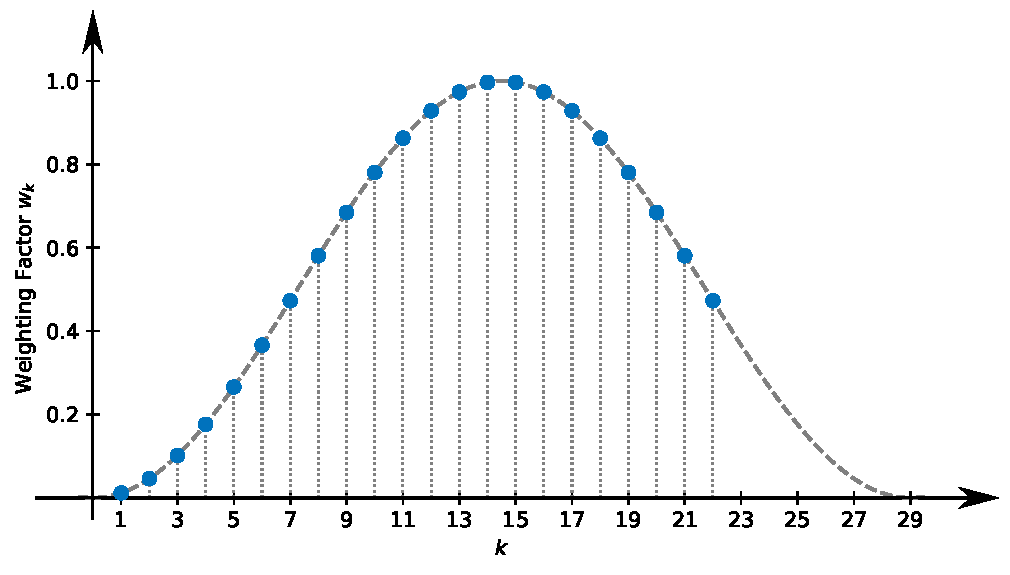
\includegraphics[width=\textwidth]{weighting_function}
  \caption{Weighting function with $n = 22$ and $N = 28$}
  \label{fig:weighting_function}
\end{figure}

% results in the weight vector w
This results in the weight vector
\begin{equation}
  \boldsymbol{w} =
  \begin{bmatrix}
    w_{1} & w_{2} & \dots & w_{n} \\
  \end{bmatrix}.
  \label{eq:weight_vector}
\end{equation}

% talk about the implementation (constant size array filed with zero)
% talk about that always the maximum amount of frames considered weights is returned (the rest is filled with zeros)
% This results in the following weight vector with $n$ elements: % $\boldsymbol{w}$
The weight vector is implemented as a fixed size one-dimensional NumPy array. % of type \texttt{np.float32}.
% The length of this array is equal to the maximum number of frames to consider, which is \num{22}.
The length of this array corresponds to the maximum number of frames to be considered, which is \num{22}.
If a throw creates less than \num{22} frames, the rest of the array is filled with zeros.
% The window function is implemented in the \texttt{sine\_squared\_window} function 
This is implemented in the \texttt{sine\_squared\_window} function, as shown in appendix \ref{app:inference_application} on line \ref{lst:ln:sine_squared_window}.

% --------------------------------------
\paragraph{Weighting of the Predictions} % Probabilities
% predictions are then weighted (reference to verificcation that shows that partial throws perform worse than fully visible ones)
% weighted average
The individual probabilities are weighted according to equation \ref{eq:weighted_probability}.

\begin{equation}
  y_k = \frac{w_1 \cdot P_{1k} + w_2 \cdot P_{2k} + \dots + w_n \cdot P_{nk}}{w_1 + w_2 + \dots + w_n} = \frac{\sum\limits_{i=1}^{n} w_i \cdot P_{ik}}{\sum\limits_{i=1}^{n} w_i}
  \label{eq:weighted_probability}
\end{equation}

where

\[
  % 1\leq k\leq c
  k = 1, 2, \dots, c
\]

and

\begin{tabular}{lll}
  $y_k$ & = & weighted probability $k$ of the weighted prediction vector $\boldsymbol{y}$ \\ % prediction
  $w_i$ & = & weighting factor $i$ of the weight vector $\boldsymbol{w}$ \\
  $P_{i,k}$ & = & probability $i,k$ of the predictions matrix $\boldsymbol{P}$ \\
  $n$ & = & number of frames considered \\
  $c$ & = & number of classes \\
\end{tabular}
\\

This results in the weighted prediction vector
\begin{equation}
  \boldsymbol{y} =
  \begin{bmatrix}
    y_{1} & y_{2} & \dots & y_{n} \\
  \end{bmatrix}.
  \label{eq:weighted_prediction_vector}
\end{equation}

% this can also be done with matrix multiplication
% done with numpy, explain the implementation and reference to it
% The actual implementation uses matrix multiplication to simplify equation \ref{eq:weighted_probability}.
The actual implementation uses matrix multiplication to perform this calculation efficiently.
Therefore, the NumPy function \texttt{np.matmul} is used to calculate the matrix product of the two arrays \cite{}. % todo: cite https://numpy.org/doc/stable/reference/generated/numpy.matmul.html
This is shown in appendix \ref{app:inference_application} on line \ref{lst:ln:matrix_multiplication}.

% todo: which version should be used?
% todo: \cdot between matrix multiplication? -> No, could be misinterpreted as the dot product
\begin{equation}
  % \boldsymbol{y} = \sum\limits_{i=1}^{n} \frac{1}{w_i} \cdot \boldsymbol{w} \boldsymbol{P}
  \boldsymbol{y} = \sum\limits_{i=1}^{n} w_i^{-1} \cdot \boldsymbol{w} \boldsymbol{P}
  \label{eq:weighted_prediction}
\end{equation}

where

\begin{tabular}{lll}
  $\boldsymbol{y}$ & = & weighted prediction vector \\ % of length $c$
  $n$ & = & number of frames considered \\
  $w_i$ & = & weighting factor $i$ of the weight vector $\boldsymbol{w}$ \\
  $\boldsymbol{w}$ & = & weight vector \\ % of length $n$
  $\boldsymbol{P}$ & = & predictions matrix \\ % $n \times c$
\end{tabular}
\\

% ------------------------------------------------------------------------------------------------------------------------------
\subsection{User Interface}
\label{subsec:inference:app:ui}
% show results (UI)

% To display the results on the screen, they have to be prepared
% The results have to be prepared to be displayed on the screen.
The results must be prepared to be displayed on the screen.
% On the one hand, a suitable frame of the throw has to be selected and on the other hand the probabilities have to be rounded
On the one hand, an appropriate frame of the captured throw has to be selected and, on the other hand, the probabilities have to be rounded and prepared in a list.

% -------------------------
\paragraph{Frame Selection}
% weighting of the frames to chose the best frame
Choosing an appropriate frame of the captured throw is done by selecting the image with the highest weighted probability of the class selected as the best prediction. % prediction made by the model
% The image with the highest weighted probability of the class selected as the best prediction is chosen.
% This corresponds to weighting the respective column of the predictions matrix $\boldsymbol{P}$, which is shown in equation \ref{eq:weighted_probabilities}.
% For this purpose the weight column vector $\boldsymbol{w}^\top$ is element-wise multiplied with 
% For this purpose, the weighted probabilities column vector $\boldsymbol{f}$ is calculated as shown in equation \ref{eq:weighted_probabilities}.
% This corresponds to the element-wise multiplication of the weight column vector $\boldsymbol{w}^\top$ with the respective column of the predictions matrix $\boldsymbol{P}$, which is shown in equation \ref{eq:weighted_probabilities}.
% For this purpose, the element-wise multiplication of the weight column vector $\boldsymbol{w}^\top$ with the respective column of the predictions matrix $\boldsymbol{P}$ is calculated, which is shown in equation \ref{eq:weighted_probabilities}.
For this purpose, the element-wise multiplication of the weight column vector $\boldsymbol{w}^\top$ with the respective column of the predictions matrix $\boldsymbol{P}$ is calculated.
This is shown in equation \ref{eq:weighted_probabilities}.
The image corresponding to the index of the highest weighted probability is then selected.
% The image corresponding to the index of the highest weighted probability, which is most likely a frame from the middle of the throw, is then selected.
% This is most likely a frame from the middle of the throw due to the applied weighting.
Due to the applied weighting, this is most likely a frame from the middle of the throw, where the object is most visible.

% todo: maybe use \odot
\begin{equation}
  \boldsymbol{f} = \boldsymbol{w}^\top \circ \boldsymbol{P}_{:,k} =
  \begin{bmatrix}
    w_{1} \cdot P_{1,k} \\
    w_{2} \cdot P_{2,k} \\
    \vdots \\
    w_{n} \cdot P_{n,k} \\
  \end{bmatrix}
  \label{eq:weighted_probabilities}
\end{equation}

where

\begin{tabular}{lll}
  $\boldsymbol{f}$ & = & weighted probabilities column vector \\
  $\boldsymbol{w}^\top$ & = & weight column vector \\
  $\boldsymbol{P}_{:,k}$ & = & column $k$ of the predictions matrix $\boldsymbol{P}$ \\
  $w_i$ & = & weighting factor $i$ of the weight vector $\boldsymbol{w}$ \\
  $P_{i,k}$ & = & probability $i,k$ of the predictions matrix $\boldsymbol{P}$ \\
  $n$ & = & number of frames considered \\
\end{tabular}
\\

The frame is then resized and encoded as a \acrshort{png}.
The implementation of the image selection and preparation process is shown in appendix \ref{app:inference_application} on lines \ref{lst:ln:frame_selection1}--\ref{lst:ln:frame_selection2}.

% ---------------------------------------
\paragraph{Rounding of the Probabilities}
% lrm round function
% The percentages are rounded to one decimal place.
% Before displaying the probabilities, they are rounded to one decimal place.
The probabilities (in percent) are rounded to one decimal place before they are displayed on the screen.
However, naively rounding percentages will quickly reveal the problem that the total value does not always add up to \SI{100}{\percent}.
The largest remainder method is used to fix this problem.
This simple method consists of the following easy three steps \cite{}: % todo: cite https://revs.runtime-revolution.com/getting-100-with-rounded-percentages-273ffa70252b
\begin{enumerate}
  \item Flooring all values
  % \item Computing the difference between the sum of the floored values and the total value
  \item Computing the difference between the total value and the sum of the floored values
  % \item Distributing this difference by adding one to each floored value until
  % \item Distributing this difference by adding one to each floored value in decreasing order of their decimal parts
  % \item Distributing the difference between the floored values in decreasing order of their decimal parts
  \item Distributing this difference by incrementing the floored values in decreasing order of their decimal parts
\end{enumerate}

% Listing \ref{lst:largest_remainder_method} shows the implementation of the largest remainder method in the \texttt{lrm\_round} function.
The largest remainder method is implemented in the \texttt{lrm\_round} function, as shown in appendix \ref{app:inference_application} on line \ref{lst:ln:lrm_round}. % done: maybe reference to appendix line xyz instead of another listing of this function?
% To round the percentages to one decimal place, the values are multiplied by ten and \num{1000} is used as the total value.
To round the percentages to one decimal place, the values are multiplied by ten before the algorithm is applied.
% As a last step, the values are divided by ten which results in percentages rounded to one decimal place.
In a final step, the values are divided by ten, resulting in percentages rounded to one decimal place.

% \begin{lstlisting}[style=python, caption={Largest remainder method}, label=lst:largest_remainder_method]
% def lrm_round(series):
%   floored_series = np.floor(series * 10.0)
%   decimal_series = series * 10.0 - floored_series
%   decimal_series_argsorted = np.argsort(decimal_series)[::-1]
%   difference = 1000 - np.sum(floored_series, dtype=np.uint16)
%   for idx in decimal_series_argsorted[0:difference]:
%     floored_series[idx] += 1
%   return_series = floored_series.astype(np.float64) / 10.0
%   return return_series.tolist()
% \end{lstlisting}
